% Start preamble
\documentclass[12pt,a4paper]{article}
\usepackage{geometry}
 \geometry{
 a4paper,
 total={170mm,257mm},
 left=20mm,
 top=20mm,
 }
\usepackage[latin9]{inputenc}
\usepackage[T1]{fontenc}
\usepackage[pdftex]{graphicx}
\graphicspath{{./}}
\usepackage{enumitem}
\usepackage{pdfpages}
\usepackage{hyperref}
\usepackage{tikz}
\usepackage{attachfile}
\usepackage{epstopdf}
\usepackage{array}
\usepackage{multirow}
\usepackage{multicol}
\usepackage{float}
%\usepackage[table]{xcolor,colorbl}
\setlength{\textwidth}{16cm}
\setlength{\oddsidemargin}{-0.5cm}
\setlength{\evensidemargin}{-0.5cm}
%\setlenght{\headsep}{0cm}
\setlength\parindent{0pt}
%\setlength{\extrarowheight}{3pt}
\usepackage{listings}
%\usepackage{xcolor}

\input{arduinoLanguage.tex}
%%%%%% Counting oppgaves %%%%%%
 \newcount\questnum \questnum=0
 \def\oppgave{
            \advance\questnum by 1
	    \ifthenelse{\questnum>0\AND \questnum<9}
	    {
                \vskip 1cm
		\textbf{Oppgave}\hskip 5pt\the\questnum \hfill \hfill(6p)
		\vskip 3pt
		\hrule
	\vskip 0.5cm}
	{
                \vskip 1cm
		\textbf{Oppgave}\hskip 5pt \the\questnum \hfill \hfill(12p)
		\vskip 3pt \hrule \vskip 0.5cm }

		}

% End preamble

\begin{document}
\title{H�stpr�ve 06 5timer}
\author{Fagl�rer: Fred-Olav Mosdal 90507684\\
Oppgave 1-8 gj�res p� ark. Hjelpemidler: kalkulator. \\
Oppgave 9 gj�res p� PC. Hjelpemidler: Alle ikke kommuniserende\\
Elektronisk del av pr�ve sendes p� email til: \\
fred-olav.mosdal@skole.rogfk.no\\
Emne: H�stpr�ve}
\maketitle
\newpage
\
\newpage
\oppgave{}% Stian sin oppgave

a) Hva er forskjellen p� en induktiv og en kapasitiv giver?
\vskip 2.5pt 

\begin{tikzpicture}
	\draw[step=0.5cm,gray!20,very thin]  grid (17,3) ;
\end{tikzpicture}
\vskip 2.5pt 
b) Hva er en NAMUR-giver, og hvordan fungerer den?
\vskip 2.5pt 

\begin{tikzpicture}
	\draw[step=0.5cm,gray!20,very thin]  grid (17,3) ;
\end{tikzpicture}
\vskip 2.5pt 
c) En komponent er merket med dette symbolet, forklar hva det betyr:
\vskip 2.5pt 

\begin{tikzpicture}
	\draw[step=0.5cm,gray!20,very thin]  grid (17,3) ;
\end{tikzpicture}
\vskip 2.5pt 
d) Tegn/forklar hva som er forskjellen p� en PNP og NPN giver
\vskip 2.5pt 

\begin{tikzpicture}
	\draw[step=0.5cm,gray!20,very thin]  grid (17,3) ;
\end{tikzpicture}
\vskip 2.5pt 
e) Forklar hvilke tre �hovedtyper� fotoelektriske (fotocelle) givere som finnes, og hvordan disse virker?
\vskip 2.5pt 

\begin{tikzpicture}
	\draw[step=0.5cm,gray!20,very thin]  grid (17,3) ;
\end{tikzpicture}
\vskip 2.5pt 
f) Nevn noen ting som er viktig � vurdere f�r du skal velge giver/sensor til et anlegg (minst 5)
\vskip 2.5pt 

\begin{tikzpicture}
	\draw[step=0.5cm,gray!20,very thin]  grid (17,3) ;
\end{tikzpicture}
\vskip 2.5pt 

Se figuren under. Tanken p� bildet skal utstyres med automatisk fylling. N�r niv�et synker under posisjonen til -S2, aktiveres magnetventilen -V1, og tanken fylles opp. N�r niv�et kommer opp til -S3, kobler magnetventilen ut. Dersom niv�et i tanken av en eller annen grunn (komponentsvikt e.l.) skulle stige opp til alarmgiveren -S4, aktiveres signallampen -P2 (og magnetventilen skal stenge). Den kapasitive giveren -S4 har en invertert utgang (NC) for p� den m�ten oppn� en selvoverv�kning av alarmkretsen (en komponentsvikt eller brudd i kabelen vil utl�se alarmen). Anlegget startes med venderen -S1, og signallampen -P1 angir at anlegget er aktivert (spenning p�). Datablad til giveren som skal benyttes finner du i vedlegget til pr�ven.

Lag styrestr�mskjema for anlegget. Tilf�rselsspenningen er enfase 230 VAC, sensorene og magnetventil er 24 VDC. Det kan benyttes hjelpereleer (ikke PLS-styring).
\oppgave{}%2 Kathrine sin oppgave
\newpage
\oppgave{}%2
\vskip 2.5pt 
Tegn en blokkskjematisk oppbyggning av en PLS med inn og utganger
\vskip 2.5pt 
\newpage
\oppgave{}%3
\vskip 25pt 
To endebrytere skal tilkobles h.h.v. \texttt{Ix.3} og \texttt{Ix.6} p� en Siemens SM-321 DI inngangsmodul(model 6ES7321-1BL00-0AA0). Tegn de n�dvendige koblingene. Det internekoblingsskjemaet for (\texttt{Ix.0}) vises som en referanse for alle inngangene.
Tegn de n�dvendige koblingene som er n�dvendig for tilkobling av endebryterene.  


$$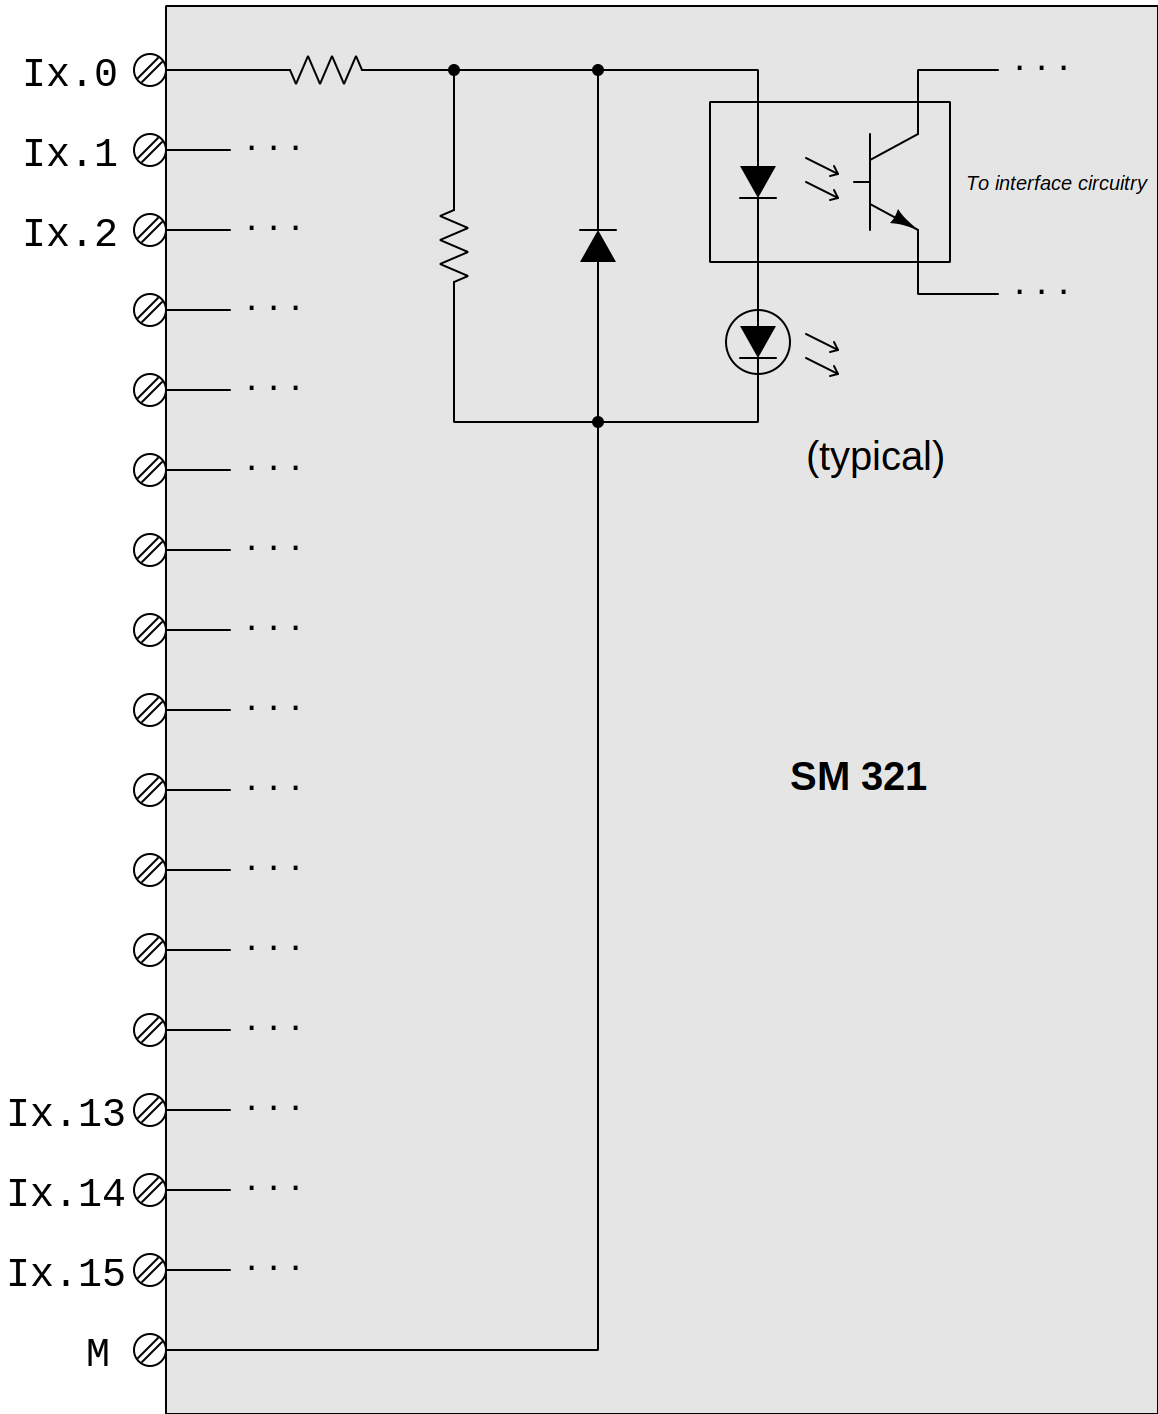
\includegraphics[width=15.5cm]{i04536x01.eps}$$

Er dette en \textit{sinking} eller en \textit{sourcing} DI modul?
\vskip 2.5pt 

\begin{tikzpicture}
	\draw[step=0.5cm,gray!20,very thin]  grid (17,1) ;
\end{tikzpicture}
\vskip 2.5pt 
\newpage
\oppgave{}%4 Lover og regler
\newpage
\oppgave{}%5 Tegne i PC|Schematic
\newpage
\oppgave{}%6 PLS programmering
\newpage
\oppgave{}%7 HMI
\newpage
\oppgave{}%8 
\oppgave{}
\vskip 2.5pt 
P� Dale stoppestasjon hender det ofte av stoppsensoren blir defekt(h�rverk). For � l�se problemet er det bestemt at en skal flytte sensoren til andre siden av gondolen. 

\vskip 10pt 
Du f�r oppdraget. Vis hvordan du ville planlagt, gjennomf�rt og dokumentert oppdraget. 


\includepdf[scale=1,pages=1,angle=90]{../output/nogpl/aAuntom05x01.pdf}

\end{document}
